\documentclass[PhD-Yoann-Dupont.tex]{subfiles}
\begin{document}

Le corpus CHEMDNER \citep{krallinger2015chemdner} est un receuil d'abstracts PubMed enrichi en entités chimiques sur lequel ont été organisées deux tâches : la première appelée CDI (Chemical Document Indexing) demandait aux concurrents, pour chaque document d'un ensemble, de donner une liste triée d'élements chimiques mentionnées dans celui-ci. Le seconde, appelée CEM (Chemical Entity Mention recognition) demandait de retrouver les différentes mentions d'entités chimiques dans un ensemble de documents. Nous nous concentrerons dans cet article sur la tâche CEM, qui décrit huit entités distinctes : les entités portant un nom de marque ou générique (TRIVIAL), les entités chimiques au nom complet (SYSTEMATIC), les abbréviations d'entités (ABBREVIATION), les formules moléculaires (FORMULA), les familles d'entités (FAMILY), les identifiants (IDENTIFIER), les groupes d'entités (MULTIPLE) et les entités dont la classe n'a pas pu être déterminée précisément (NO\_CLASS). Une fiche récapitulative du corpus est donnée dans la figure\ \ref{tab:chemdner-recap-card}, tandis que des exemples d'entités sont donnés dans la figure\ \ref{fig:CHEMDNER-examples}.

\begin{table}[ht!]
\centering
\begin{tabular}{|p{0.21\linewidth}|p{0.21\linewidth}|p{0.21\linewidth}|p{0.21\linewidth}|}
\hline
\multicolumn{4}{|c|}{\textbf{corpus CHEMDNER}} \\
\hline
\multicolumn{2}{|c|}{\textbf{général}} & \multicolumn{2}{c|}{\textbf{annotations}} \\
\hline
\textbf{type de texte} & articles scientifiques & \textbf{niveaux d'analyse} & $\emptyset$ \\
\hline
\textbf{unités d'analyse} & document,\newline titre,\newline résumé & \textbf{structuration} & conjonction* \\
\hline
\textbf{volume texte brut} & 13.7 Mo & \textbf{types\newline d'entités} & 8 \\
\hline
\textbf{format} & xml (annotations externalisées) & \textbf{entités inconnues} & 39.45\% \\
\hline
\textbf{langue(s)} & Anglais & \textbf{accord inter-\newline annotateurs}** & 0.8526 \\
\hline
\end{tabular}
\scriptsize{\\ *éléments spécifiques de la conjonction non disponibles}
\scriptsize{\\ **il ne s'agit pas d'un $\kappa$, mais d'un taux d'accord.}
\caption{Fiche récapitulative du corpus CHEMDNER pour la tâche CEM}
\label{tab:chemdner-recap-card}
\end{table}

Une description condensée du corpus est disponible dans le tableau \ref{tab:chemdner-splits-numbers}. Nous pouvons également ajouter qu'environ 10000 entités du test sont inconnues du corpus de train (39,45\%). Ce nombre baisse à 8400 si on considère les corpus d'entrainement et de développement (33,13\%). Ce nombre d'entités inconnues est presque le double de ce que l'on peut trouver pour des corpus en entités nommées plus classiques, ce qui illustre bien l'une des difficultés de cette tâche, à savoir la grande taille du vocabulaire. L'exemple donné dans la figure\ \ref{fig:CHEMDNER-examples} exemplifie la raison principale de ce fort taux d'entités inconnues : le côté combinatoire des entités d'un point de vue morphologique, cette grande variance causant un grand nombre de formes différentes sur les entités.

\begin{figure}[ht!]
\begin{helvetica}
\small
Two new \textcolor{purple}{[FAMILY spirostanols]} and a new \textcolor{red}{[TRIVIAL furostanol]}, \textcolor{brown}{[MULTIPLE reinocarnoside A (1), B (2) and C (3)]}, were isolated from the roots of Reineckia carnea, together with two known compounds, \textcolor{blue}{[SYSTEMATIC (25S)-1$\beta$,3$\beta$,4$\beta$-trihydroxyspirostan-5$\beta$-yl-O-$\beta$-D-glucopyranoside]} (4), \textcolor{blue}{[SYSTEMATIC kitigenin-5$\beta$-O-$\beta$-D-glucopyranoside]} (5). \\
$[$...$]$ their anticancer activities were evaluated by \textcolor{green!50!black}{[ABBREVIATION MTT]} method. \\
$[$...$]$ from site-controlled \textcolor{orange}{[FORMULA In(Ga)As]}/\textcolor{orange}{[FORMULA GaAs]} quantum dots. \\
$[$...$]$ the \textcolor{purple}{[FAMILY cyclic pentapeptide]} \textcolor{teal}{[IDENTIFIER FC131]}, peptide mimetics, and \textcolor{purple}{[FAMILY dipicolylamine]}-containing compounds were designed and synthesized.
\end{helvetica}
\caption{Des exemples d'entités corpus CHEMDNER}
\label{fig:CHEMDNER-examples}
\end{figure}

\begin{comment}
\begin{figure}[ht!]
    \centering
    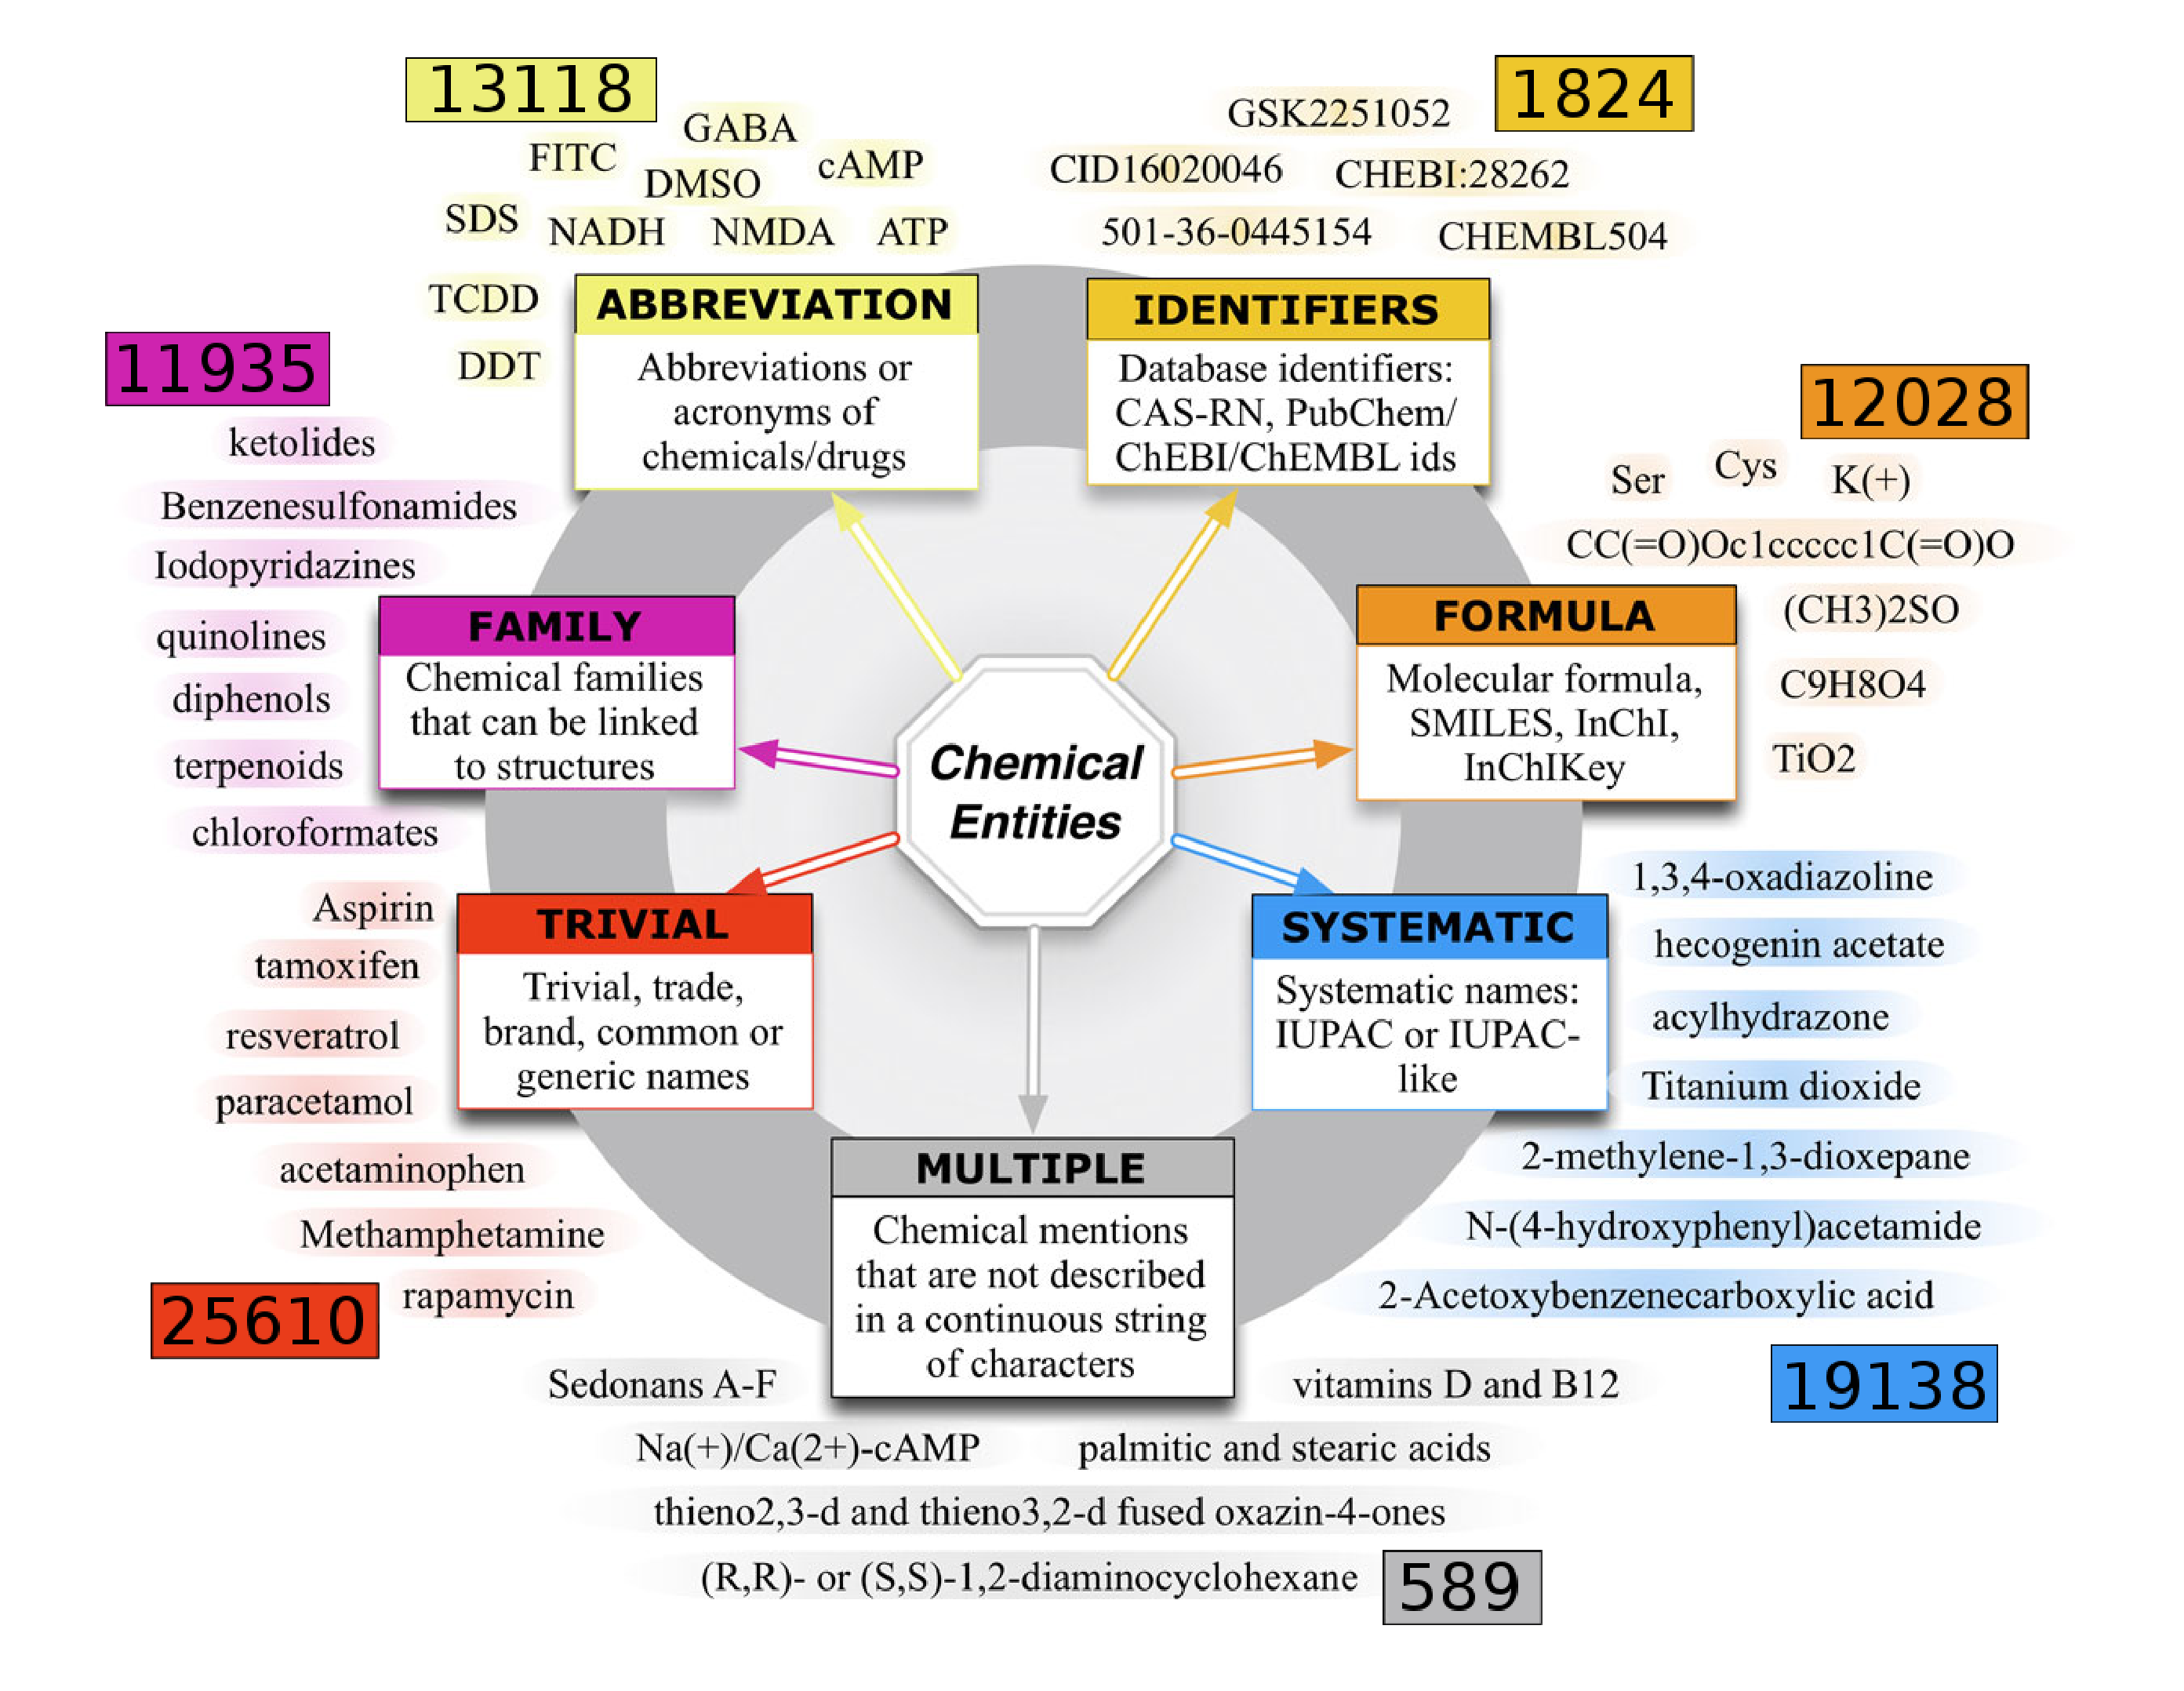
\includegraphics[scale=0.225]{images/corpus/CHEMDNER/CHEMDNER-entities-counts}
    \caption{une vue d'ensemble des entités corpus CHEMDNER}
    \label{fig:CHEMDNER-counts}
\end{figure}
\end{comment}

\begin{table}[ht!]
\centering
\begin{tabular}{|l|c|c|c|}
\cline{2-4}
\multicolumn{1}{c|}{} & train & dev   & test   \\
\hline
documents             & 3500  & 3500  & 3000   \\
entités               & 26478 & 29526 & 25351  \\
\hline
TRIVIAL               & 8832  & 8970  & 7808   \\
SYSTEMATIC            & 6656  & 6816  & 5666   \\
ABBREVIATION          & 4538  & 4521  & 4059   \\
FORMULA               & 4448  & 4137  & 3443   \\
FAMILY                & 4090  & 4223  & 3622   \\
IDENTIFIER            & 672   & 639   & 513    \\
MULTIPLE              & 202   & 188   & 199    \\
NO\_CLASS             & 40    & 32    & 41     \\
\hline
\end{tabular}
\caption{description brève du corpus CHEMDNER pour la tâche CEM}
\label{tab:chemdner-splits-numbers}
\end{table}

Le corpus CHEMDNER a pour avantage d'être très large et d'avoir un très fort taux d'accord inter-annotateurs, ce dernier atteignant 91\%. Son inconvénient principal étant les entités de type MULTIPLE, qui sont en fait des conjonctions d'entités, cette structuration n'étant pas prise en compte par les annotateurs. Autrement dit, les entités spécifiques composant une entité MULTIPLE ne sont pas annotées dans le corpus, ne permettant pas de les repérer de façon simple.

\end{document}